%!TEX root = main.tex
\afterpage{\blankpage}
\newpage
\chapter{Experimentálne overenie}
\label{sec:experiment}

Navrhnutú metódu vytvárania personalizovaných informačných bulletinov sme sa rozhodli overiť prostredníctvom
nekontrolovaného online experimentu. Väčšina prác venujúcich sa odporúčaniu v doméne CQA systémov overuje
svoje hypotézy v offline experimentoch na kontrolovaných vzorkách dát. Pre účely realistického overenia našej metódy, hlavne
z pohľadu faktorov špecifických pre informačné bulletiny, však overovanie v offline experimente nie je dostačujúce.
Online nekontrolované experimenty samozrejme vyžadujú oveľa viac námahy a ich výsledky nie sú garantované, no v prípade,
že je takýto experiment úspešný, má oveľa väčší potenciál priniesť relevantné výsledky.

Experiment sme vykonávali na používateľoch z komunity Stack Overflow platformy Stack Exchange.
Komunitu Stack Overflow sme pre náš experiment zvolili z viacerých dôvodov, hlavne však preto,
že sa jedná o jednoznačne najaktívnejšiu komunitu z celej platformy, v ktorej bol najväčší potenciál získať čo najviac
používateľov do nášho experimentu. Okrem toho zohrával úlohu v rozhodovaní aj fakt, že táto komunita sa venuje doménovej
oblasti, v ktorej máme určité vedomosti, čo nám umožňilo jednoduchšie odhadnúť úroveň relevancie odporúčaného obsahu.

Do experimentu sa mohli prihlásiť všetci používatelia, ktorí majú konto na portáli Stack Overflow, prostredníctvom
registračného formuláru systému StackLetter. Celkovo sa nám podarilo získať pomerne diverznú vzorku používateľov,
medzi ktorými boli prítomní okrem iných aj úplni nováčikovia bez akejkoľvek predošlej aktivity, ale aj mimoriadne aktívni
a dlhodobo rešpektovaní členovia komunity. Používatelia mali pri registrácii možnosť vybrať si buď denný alebo týždenný
informačný bulletin. Túto voľbu tiež mohli kedykoľvek počas experimentu zmeniť.

\textbf{TODO} -- GRAF - podiel daily/weekly subscriberov.

\section{Metodológia experimentu}
Experiment prebiehal formou A/B testovania. Na rozdiel od štandardného A/B testovania, v ktorom sa používatelia rozdelia
do dvoch alebo viacerých skupín, sme náš test vykonávali na báze striedania použitých metód v časových intervaloch:

\begin{adjustwidth}{1cm}{1cm}
\textbf{1. Kontrolná skupina}\\
V prvej fáze experimentu, od 9. novembra 2017 do 11. marca 2018, sme používateľom generovali informačný bulletin len
prostredníctvom triviálnej metódy odporúčania, ktorá vyberala otázky označené značkami, v ktorých v minulosti používateľ
položil otázku, ponúkol odpoveď alebo okomentoval príspevok. Dáta z tejto skupiny slúžili ako počiatočné dáta pre porovnanie
s ostatnými metódami.

Od 12. marca 2018 sme nasadili metódy vytvárania odporúčaní opisované v tejto práci. Metódy generovania informačných bulletinov
sa striedali na týždennej báze.

\textbf{2. Metóda A -- Personalizované odporúčanie}\\
Využívala sa metóda personalizovaného odporúčania opísaná v kapitole~\ref{impl:pers-method}, pričom sa aplikovala
metóda pre zabezpečenie aktuálnosti odporúčaného obsahu. V tomto prípade sa nevykonávala žiadna diverzifikácia odporúčaní.

\textbf{3. Metóda B -- Personalizované odporúčanie s diverzifikáciou}\\
V tomto prípade sa zostavovali personalizované informačné bulletiny s využitím diverzifikačnej metódy tématického
vzorkovania, ako aj metódy pre zabezpečenie aktuálnosti odporúčaného obsahu.
\end{adjustwidth}

A/B testovanie formou striedania metód nám umožnilo vyhnúť sa problému s nerovnomerne rozloženými používateľmi v jednotlivých
skupinách z pohľadu ich aktivity, a tiež nespôsobilo problém pri postupne sa vyvíjajúcom počte používateľov.
Naopak ako potencíalny problém, s~ktorým treba pri takomto riešení počítať, sa ukázalo prirodzené postupné znižovanie
záujmu a~aktivity používateľov počas trvania experimentu.


\section{Metriky hodnotenia výsledkov}

Pre overovanie výsledkov experimentov sme využili nasledovné metriky:

\textbf{Precision@N}\\
Presnosť (angl.~\emph{Precision}), alebo tiež \textit{pozitívna predikčná hodnota} je metrika reprezentujúca pomer relevantných
dokumentov z celkového zoznamu. Štandardne sa presnosť počíta ako pomer z celého zoznamu dokumentov, no v oblasti
odporúčania a vyhľadávania informácií je často vhodnejšou odvodená metrika \textit{Precision@N}, ktorá určuje, aká časť
z prvých N dokumentov v~zozname odporúčaní je pre používateľa relevantná.
$$\mbox{Precision@N}=\frac{|\{\mbox{relevantne otazky v top-N}\}\cap\{\mbox{top-N odporucenych otazok}\}|}
{|\{\mbox{top-N odporucenych otazok}\}|}$$

\textbf{DCG}\\
\textit{Discounted Cumulative Gain} je metrika kvality ohodnocovania často používaná na meranie efektívnosti
odporúčania. DCG meria užitočnosť dokumentov na základe ich pozície vo výslednom zozname. Užitočnosť dokumentov sa akumuluje
od konca zoznamu, pričom najvyššiu užitočnosť majú dokumenty na začiatku zoznamu~\cite{Jrvelin2002}.

DCG položky na pozícii $p$ v zozname odporúčaní je definované ako:

$$\mathrm{DCG_{p}} = \sum_{i=1}^{p} \frac{ 2^{rel_{i}} - 1 }{ \log_{2}(i+1)}$$
\begin{adjustwidth}{1cm}{1cm}
$rel_i$ -- relevancia $i$-tej položky v zozname odporúčaní.\\
\end{adjustwidth}

\textbf{CTR a používateľská aktivita}\\
Miera preklikov (angl.~\emph{Click-through Rate}) je metrika často využívaná v spojitosti s informačnými bulletinmi.
Táto metrika vyjadruje počet úspešných kliknutí na odkaz v informačnom bulletine. V našom experimente sme za úspešné
považovali kliknutia na samotné položky alebo poskytnutie pozitívnej spätnej väzby na položku.

Okrem miery úspešných preklikov sme využili aj odvodenú metriku používateľskej aktivity, ktorá vyjadruje celkový počet
kliknutí na akékoľvek odkazy v informačnom bulletine.

\textbf{Predpoklady výsledkov metrík}\\
Na základe našich hypotéz sme predpokladali nárast vo všetkých sledovaných metrikách pri porovnávaní metódy personalizovaného
odporúčania s kontrolnou skupinou. Pri porovnávaní diverzifikovaného odporúčania a personalizovaného odporúčania sme
predpokladali čiastočný pokles metrík relevancie odporúčaní (Precision@N, DCG), no nárast metrík používateľskej aktivity
-- CTR, impresie, konverzie.


\section{Vyhodnotenie výsledkov experimentu}

\textbf{Presnosť odporúčaní -- Precision@N}\\
Podľa očakávania dosiahla metóda personalizovaného odporúčania výrazne lepšie výsledky pozitívnej predikčnej hodnoty
ako triviálne odporúčanie (viď tabuľka~\ref{tab:pan}), konkrétne približne dvojnásobné. Rovnako podľa očakávania mala
metóda diverzifikácie za dôsledok zníženie presnosti odporúčaní, ktoré však boli aj naďalej výrazne lepšie,
ako v prípade triviálnej metódy.

\begin{table}[H]
\centering
\caption{Priemerné hodnoty Precision@N.}
\label{tab:pan}
\begin{tabular}{|l|c|c|c|c|c|}
\hline
                           & \textbf{N = 1} & \textbf{N = 2} & \textbf{N = 3} & \textbf{N = 4} & \textbf{N = 5} \\ \hline
\textbf{Kontrolná skupina} & 0.0266         & 0.0235         & 0.0233         & 0.0232         & 0.0230         \\ \hline
\rowcolor[HTML]{32CB00}
\textbf{Metóda A}          & 0.0546         & 0.0506         & 0.0485         & 0.0449         & 0.0473         \\ \hline
\textbf{Metóda B}          & 0.0361         & 0.0356         & 0.0301         & 0.0292         & 0.0274         \\ \hline
\end{tabular}
\end{table}


\textbf{Užitočnosť odporúčaní -- DCG}\\
Metriku DCG sme pre triviálnu metódu odporúčania nepočítali, nakoľko táto metóda nepočítala konkrétne hodnoty relevancie
jednotlivých položiek. Dopad diverzifikačnej metódy tématického vzorkovania na celkovú užitočnosť zoznamu odporúčaní sa ukázal
ako zanedbateľný.

\begin{table}[H]
\centering
\caption{Priemerné hodnoty DCG na pozícii $p$.}
\label{tab:dcgn}
\begin{tabular}{|l|c|c|c|c|c|}
\hline
                  & \textbf{p = 1} & \textbf{p = 2} & \textbf{p = 3} & \textbf{p = 4} & \textbf{p = 5} \\ \hline
\rowcolor[HTML]{32CB00}
\textbf{Metóda A} & 1.02           & 1.66           & 2.17           & 2.61           & 3.00           \\ \hline
\textbf{Metóda B} & 1.01           & 1.65           & 2.16           & 2.60           & 2.98           \\ \hline
\end{tabular}
\end{table}


\textbf{Spokojnosť používateľov -- CTR a používateľská aktivita}\\
\textbf{TODO}, v skratke:\\
-- Hypoteza 1 sa potvrdila, pouzivatelia preferuju personalizovany newsletter, CTR je takmer 2.5x, Aktivita takmer 3.5x\\
-- Hypoteza 2 sa nepotvrdila, pouzivatelia vnimaju diverzifikaciu negativne, z toho vyplyva zvysene mnozstvo negativnej spatnej vazby
a znizenie urovne CTR (voci personalizovanemu). Stale lepsie ako nepersonalizovane/trivialne.\\
-- Udaje su statisticky signifikantne, vid. analyza rozptylu - ANOVA.\\
Z toho vyplyva: pouzivatelia maju radi filtracnu bublinu v pripade newslettrov. (Ale negeneralizovat privelmi!)

\begin{table}[H]
\centering
\caption{Priemerné hodnoty CTR a používateľskej aktivity.}
\label{tab:ctr}
\begin{tabular}{|l|c|c|}
\hline
                           & \textbf{CTR} & \textbf{\begin{tabular}[c]{@{}c@{}}Používateľská\\ aktivita\end{tabular}} \\ \hline
\textbf{Kontrolná skupina} & 0.024        & 0.036             \\ \hline
\rowcolor[HTML]{32CB00}
\textbf{Metóda A}          & 0.058        & 0.123             \\ \hline
\textbf{Metóda B}          & 0.034        & 0.098             \\ \hline \hline
\multicolumn{3}{|c|}{\textbf{ANOVA}}                          \\ \hline
\textbf{F-value}           & 12.69        & 34.14             \\ \hline
\textbf{P-value}           & $3×10^{-6}$  & $2×10^{-15}$      \\ \hline
\end{tabular}
\end{table}


\subsection{Aktivita používateľov}

Aktivita používateľov v informačnom bulletine sa ukázala ako problémový faktor nášho experimentu. Veľká časť používateľov
bola totiž aktívna iba počas prvých dní alebo týždňov od registrácie, a ich aktivita postupom času klesala, ako to
naznačuje aj trendová čiara v grafe~\ref{fig:user-act-hist}.
Napriek tomu sa nám podarilo získať dostatočné množstvo dát o aktivite používateľov na to, aby sme vyhodnotili úspešnosť
experimentu (viď tabuľka~\ref{tab:user-act}).

\begin{table}[h]
\centering
\caption{Štatistika používateľskej aktivity v online experimente.}
\label{tab:user-act}
\begin{tabular}{|m{7cm}|>{\raggedleft\arraybackslash}m{2.5cm}|}
\hline
\textbf{Štatistika} & \textbf{Počet}      \\\hline
Odoberatelia                      &   40  \\\hline
Odoslané informačné bulletiny     & 2400  \\\hline
Otvorené informačné bulletiny     &  750\footnotemark  \\\hline
Celkový počet otvorení bulletinov & 1050  \\\hline
Implicitná spätná väzba           &  530  \\\hline
Explicitná spätná väzba           &  960  \\\hline
Explicitná spätná väzba           &  960  \\\hline
Odhlásenia informačného bulletinu &    3  \\\hline
\end{tabular}
\end{table}

\begin{figure}[H]\begin{center}
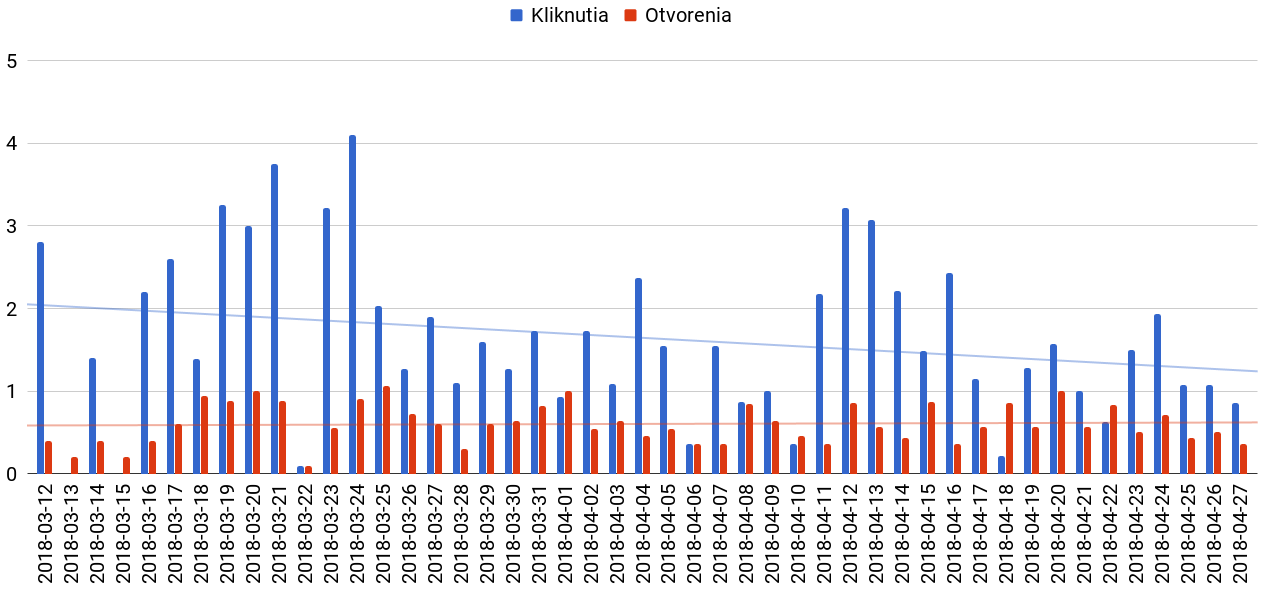
\includegraphics[scale=0.37]{user-activity-hist}
\caption{Priemerná aktivita používateľov v jednotlivých dňoch. \label{fig:user-act-hist}}\end{center}
\end{figure}

\footnotetext{Počet otvorení informačného bulletinu môže byť skreslený, nakoľko viaceré e-mailové klienty blokujú
zobrazenie obrázkov použitých na vyhodnotenie otvorenia e-mailu. Jedná sa tak o spodnú hranicu reálneho počtu.}


\subsection{Dotazník odoberateľov}

\textbf{TODO}\\
-- Odpovedalo 27.5\% odoberatelov\\
-- Obsah sa im pacil, 63\% si vsimlo personalizaciu, vsetci ju povazuju za useful.\\
-- Nevedia velmi posudit ci bol pre nich obsah relevantny (63\% dalo strednu hodnotu), len 4 dali vyssiu.\\
-- Vsetci povazuju personalizovane newslettre za very good idea\\
-- 70\% sa priznalo ze neboli zrovna aktivni (2-4/10), 45\% si mysli ze boli relativne aktivni (7-8/10), nikto sa nesiel pretrhnut (8+).\\
-- Samozrjeme vysledky mozu byt do urcitej miery skreslene, kedze neaktivni nevyplnaju ani dotaznik.
